\documentclass{beamer}
\usetheme{Boadilla}
\usecolortheme{whale}
\setbeamertemplate{navigation symbols}{}
\setbeamertemplate{sections/subsections in toc}[sections numbered]

%Information to be included in the title page:
\title{Fuzz testing in hardware verification}
\author{Hossein Afkar}
\institute{University Of Tehran}
\date{\today}

\begin{document}

\frame{\titlepage}

\begin{frame}
    \frametitle{Table of Contents}
    \tableofcontents[hideallsubsections]
\end{frame}

\AtBeginSection[]
{
    \begin{frame}{Outline}
        \tableofcontents[currentsection, currentsubsection]
    \end{frame}
}

\section{An Introduction To Fuzz Testing}
\subsection{What is Fuzz Testing}
\begin{frame}{What is Fuzz Testing}
    \frametitle{Fuzz Testing}
    \begin{block}{Fuzz Testing}
        Software fuzzing is an automated testing technique designed to identify
        security vulnerabilities in software. It involves three steps.
        \begin{itemize}
            \item Test generation using fuzzy input
            \item Monitoring test execution
            \item Crash triaging
        \end{itemize}
    \end{block}
    Fuzz testing dates back to the 1995 but really took off when AFL(American
    Fuzzy Lop) was released.
\end{frame}

\begin{frame}
    \frametitle{Sample Bugs}
    \begin{itemize}
        \item Timeouts
        \item Interger Overflows
        \item Out Of Memory
        \item Null Dereference
        \item Assertions
        \item Buffer Overflows
        \item Stack Overflows
        \item Memory Leaks
    \end{itemize}
\end{frame}

\begin{frame}
    \frametitle{Example Of An Software Fuzzer}
    \begin{itemize}
        \item AFL(Americal Fuzzy Lop)
        \item OSS-Fuzz
        \item Special Case Fuzzing
            \begin{itemize}
                \item Creating enviornment for the program like the verification
                    environment for the hardware
            \end{itemize}
    \end{itemize}
\end{frame}

\subsection{Fuzzing Glossary}
\begin{frame}
    \frametitle{Fuzzing Glossary}
    \begin{description}[Mutation Engine]
        \item[Corpus] A set of test inputs
        \item[Cross Pollination] Using a corpus of another target to extend
            out target
        \item[Dictionary] Specifing interesting targets for fuzzing
        \item[Fuzz Target] A function to which we apply fuzzing
        \item[Fuzzing Engine] A tool that tries to find interesting input for
            a fuzz target by executing it
        \item[Mutation Engine] A tool that gets a set of testcases as input and
            creates their mutated versions
    \end{description}
\end{frame}

\begin{frame}
    \frametitle{Fuzzing Glossary}
    \begin{description}[Test Generator]
        \item[Reproducer] Or a test case is an input that can be used to
            reproduce a bug
        \item[Sanitizer] A dynamic testing tool that can detect bugs during
            runtime like ASAN
        \item[Seed Corpus] A small initial corpus with the intent of providing
            initial coverage for fuzzing
        \item[Test Generator] A tool that generates test cases according to
            some rules or grammer
        \item[Test Input] A sequence of bytes used as input to the fuzz target
        \item[Harness] A test case or a particular test target
    \end{description}
\end{frame}

\section{Using Software Fuzzing Methods In Hardware}
\begin{frame}
    \frametitle{Challenges and Required Adaptations}
    \begin{enumerate}
        \item Interface with HSB(Hardware Simulation Binary)
            \begin{itemize}
                \item Contain other components beside the DUT
                \item Require different initializations
            \end{itemize}
        \item Account for the difference between the software and hardware
            input
        \item Design a general-purpose fuzzing harness and a suitable grammar
            that ensures meaningful mutations
    \end{enumerate}
\end{frame}

\subsection{Approach}
\begin{frame}
    \frametitle{Approach}
    Approach that has been taken with the fuzzing hardware like software paper
    is divided into three steps.
    \begin{itemize}
        \item Translating Hardware To Software
        \item Hardware Coverage Tracing
        \item Interpreting Fuzzer-Generated Tests
    \end{itemize}
\end{frame}

\begin{frame}
    \frametitle{Translating Hardware To Software}
    \begin{block}{Verilator}
        Verilator is a compiler that translates hardware design to a
        cycle-accurate C++ model for fuzzing. \\
        To interface with this model verilator exposes class members for each
        input/output of the top level design. Calling the function
        \textit{eval} causes the model to operate for half a cycle.
    \end{block}
\end{frame}

\begin{frame}
    \frametitle{Hardware Simulation Binray}
    \begin{figure}
        \centering
        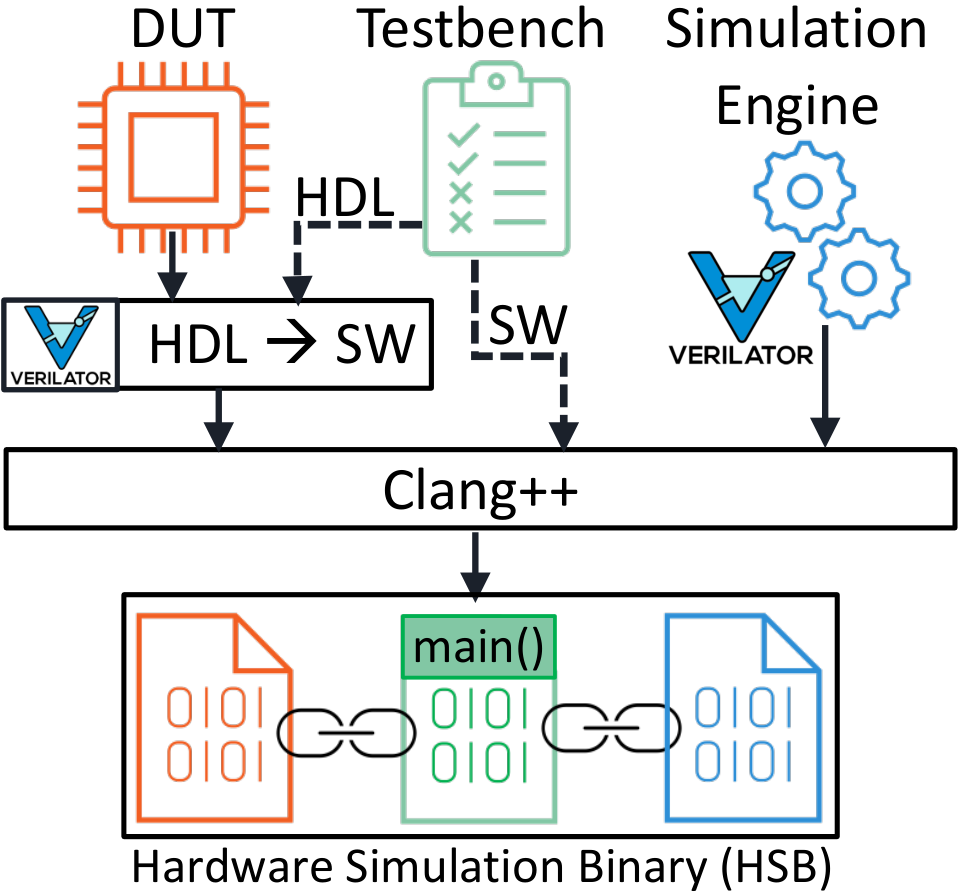
\includegraphics[width=0.5\textwidth]{hsb.png}
        \caption{Example of Hardware Simulation Binary using Verilator}
        \label{fig:hsb}
    \end{figure}
\end{frame}

\begin{frame}
    \frametitle{Hardware Coverage Tracing}
    In order to explore the DUT's state space we should use the Coverage
    Directed Generation techniques. There are two main categories of coverage
    metrics used in hardware verification.
    \begin{enumerate}
        \item Code Coverage
        \item Functional Coverage
    \end{enumerate}
    \textcolor{red}{Regardless of the method used, tracing HDL coverage is
    slow since coverage traced in the software (simulation) domain must be
    mapped back to hardware}
\end{frame}

\begin{frame}
    \frametitle{Interpreting Fuzzer-Generated Tests}
    As for software an input activates an entire set of state transitions with
    the program. But in an HSB a sequence of inputs is required to activate.
    state transition in the program \\
    We should map a single dimentional fuzzer-generated test to two dimentions;
    space and time.
\end{frame}

\subsection{Implementation}
\begin{frame}
    \frametitle{Implementation}
    Verilator and fuzzer-provided compilers (like afl++-clang) already provide
    solutions to the first components of this approach that is hardware to
    software translation and coverage tracing.
\end{frame}

\begin{frame}
    \frametitle{Bus-Centric Harness}
    Because the multi-dimentional fuzzing harness described in the past slides
    is not design agonistic this paper suggests that fuzzing should occur at
    the bus interface between the IP cores. \\
    \textcolor{red}{Naturally this is true if we have a bus. if we do not have
    a bus we should design our own harness and give an interface for the
    software fuzzer to mutate bytes}
\end{frame}

\begin{frame}
    \frametitle{Example Of An Simple Configurable Lock}
    \begin{figure}
        \centering
        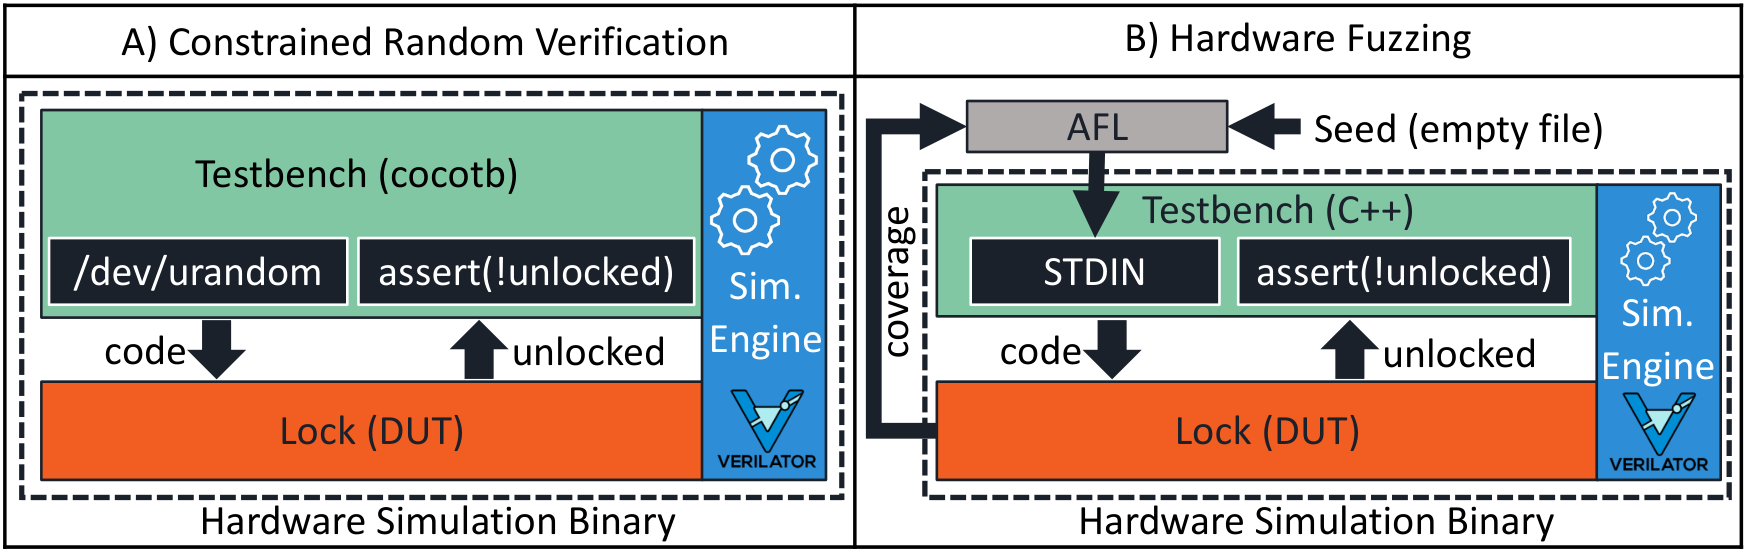
\includegraphics[width=1.0\textwidth]{lock.png}
        \caption{This shows a digital lock architecture of the HSB that this
        paper used to show how this approach works with different types of 
        fuzzing methods and how they can use the existing methods in software
        fuzzing world to improve performance of the fuzzer}
        \label{fig:lock}
    \end{figure}
\end{frame}

\section{RFuzz: Another Form Of Hardware Fuzzing}
\begin{frame}
    \frametitle{RFuzz}
    Another method that can be classified as fuzzing in the hardware is the
    RFuzz which tries to implement ideas from software fuzzing in the hardware
    but not by implementing them on hardware and thus using a FPGA.
\end{frame}

\subsection{Introduction}
\begin{frame}
    \frametitle{Coverage-Directed Mutational Fuzz Testing}
    Ideas used in the RFuzz are based on the AFL. This fuzzer consists of three
    components
    \begin{itemize}
        \item Fuzz server that snapshots the program
        \item Static or dynamic runtime instrumentation that runs the specified
            harness
        \item Fuzz engine that implements the input selection and mutation
    \end{itemize}
\end{frame}

\subsection{Approach}
\begin{frame}
    \frametitle{Input Definition}
    \begin{figure}
        \centering
        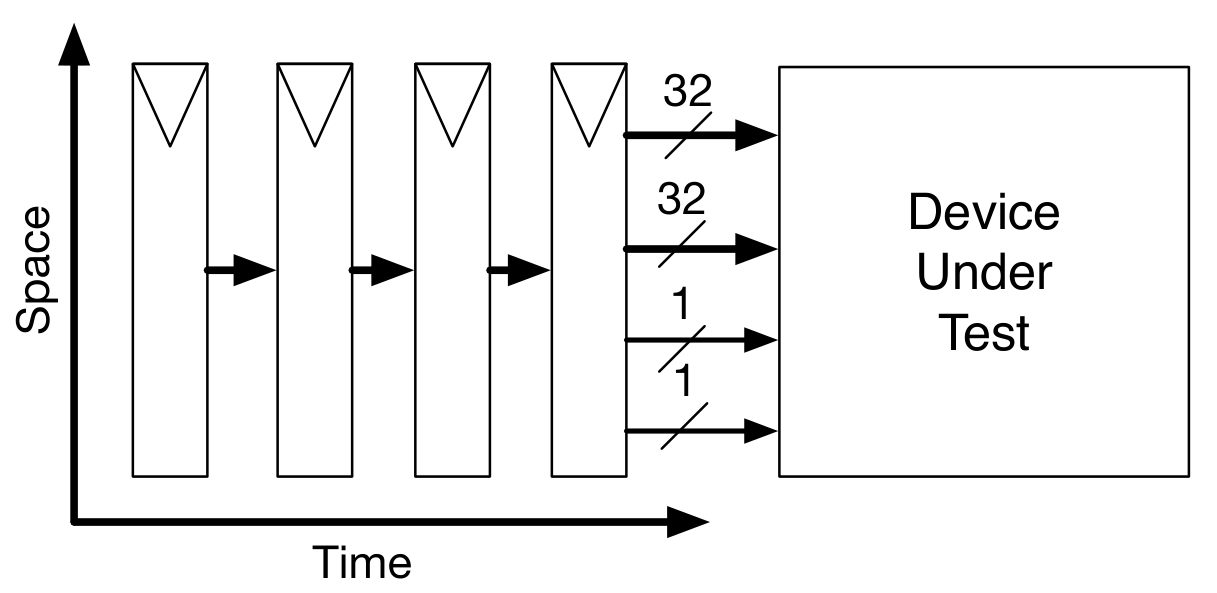
\includegraphics[width=1.0\textwidth]{input.png}
        \caption{In order for the fuzz engine to mutate the bytes we need to
        concatenate the input pins into a bit vector thus making the inputs
        into a series of bytes. Then we concatenate each cycle inputs into a
        single multi-byte input.}
        \label{fig:input}
    \end{figure}
\end{frame}

\begin{frame}
    \frametitle{Deterministic Test Execution}
    In order for the test to be deterministic and repeatable, fuzz testing
    should be started from a known state. Thus a test should be reproducible as
    long as the test inputs are known. \\
    In the following section these issues regarding FPGA resetting is addressed
    \begin{itemize}
        \item For efficiency reason many registers are not reinitialized during
            device reset
        \item Memories do not feature reset circuitry and can only be
            initialized one word at a time
    \end{itemize}
\end{frame}

\begin{frame}
    \frametitle{Register Meta Reset}
    In order to prevent the undeterministic behaviour of the registers initial
    value and the lack of register reset mechanisms this paper suggests two
    methods
    \begin{itemize}
        \item Treat inital register value as a part of the input
        \item Reset all registers to a predefined value before each test
    \end{itemize}
    This paper chooses the second method and adds a \textit{MetaReset} wire
    too initialize the value to zero in an IR pass and then the \textit{reset}
    line initializes the value to the designer intended value.
\end{frame}

\begin{frame}
    \frametitle{Sparse Memory}
    Memories are rarely meant to be reset during DUT initialization. \\
    In order to reset the memory state back to state it was before the
    execution of the test, all writes are kept track of and after
    the test values are reset to the ones before the test.
\end{frame}

\begin{frame}
    \frametitle{Coverage}
    We need a coverage metric to measure how well the mutational fuzz testing
    is working. \\
    In order to not limit the definition to the common HDL
    languages, this paper used the mux control coverage which treats every
    2:1 multiplexer as a cover point. for a mux to be covered it needs to be
    true and false during a single test.
\end{frame}

\begin{frame}
    \frametitle{Mutation Algorithm}
    Similar to the AFL, every new entry in the test set is first mutated
    with the deterministic mutation technique listed in the paper. Once we run
    out of the deterministic mutations we switch to the \textit{havoc} stage
    which makes use of the mutations that are not determinstic and might
    change the input array size.
\end{frame}

\subsection{Implementation}
\begin{frame}
    \frametitle{Implementation and Instrumentation}
    The tool \textit{RFuzz} first translates the design to the intermediate
    language called \textit{FIRRTL}. \\
    After this stage passes can be run on the source HDL to prepare it for
    the fuzz testing and implement all the details described by the previous
    slides.
\end{frame}

\begin{frame}
    \frametitle{Test Harness Generation}
    The test harness generator creates a wrapper for any RTL design by
    consuming the target design information, including inputs and coverage pins
    generated.
\end{frame}

\begin{frame}
    \frametitle{Fuzz Engine}
    \begin{figure}
        \centering
        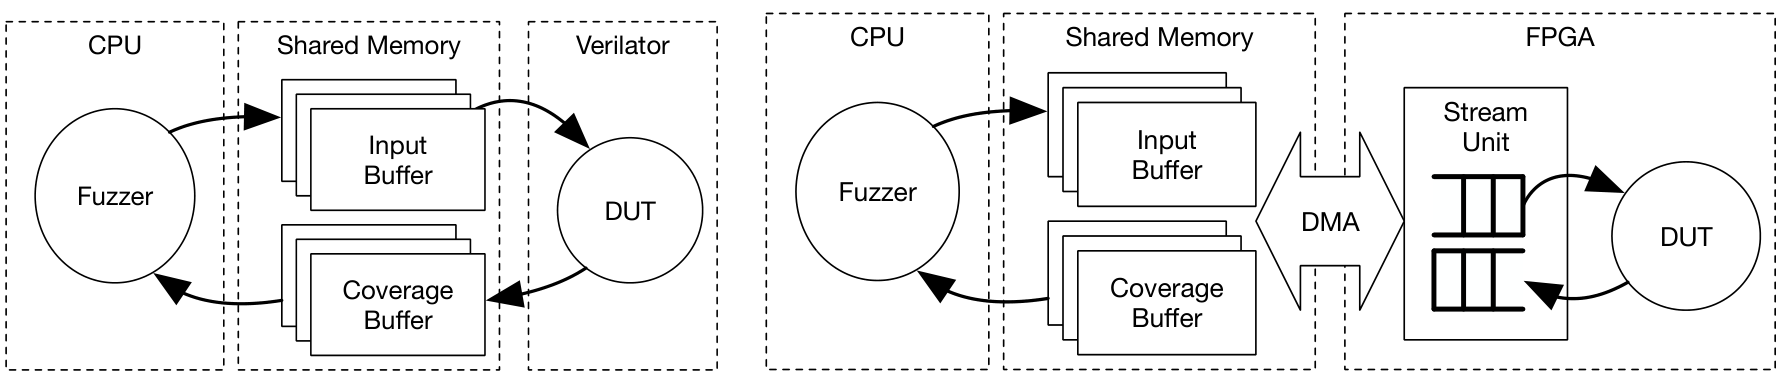
\includegraphics[width=1.0\textwidth]{rfuzz.png}
        \caption{The DUT and coverage pins are synthesized on the FPGA,
        while the coverage analysis and input generation are handled on a cpu}
        \label{fig:rfuzz}
    \end{figure}
\end{frame}

\section{RFuzz vs Fuzzing Hardware on Software}
\begin{frame}
    \frametitle{Comparison}
    \begin{itemize}
        \item RFuzz needs explicit knowledge about the DUT to generate design
            specific harness.
        \item RFuzz runs on FPGA which means faster running time. note
            that this may not be true using verilator multicore running engine.
        \item RFuzz uses a custom fuzzer based on the AFL while Fuzzing
            Hardware on Software is not limited to AFL.
    \end{itemize}
\end{frame}

\end{document}
